\documentclass{report}
\usepackage{geometry}
\usepackage{amssymb}
\usepackage{fancyhdr}
\usepackage{multicol}
\usepackage{blindtext}
\usepackage{color}
\usepackage[fontsize=16pt]{fontsize}
\usepackage{lipsum}
\usepackage{pgfplots}
\usepackage{physics}
\usepackage{mathtools}

\setlength{\columnsep}{1cm}
\def\columnseprulecolor{\color{blue}}
\date{Fall 2023}

\newcommand{\textoverline}[1]{$\overline{\mbox{#1}}$}


\title{MATH241}
\author{Aiden Sirotkine}

\begin{document}

\pagestyle{fancy}
\maketitle
\clearpage


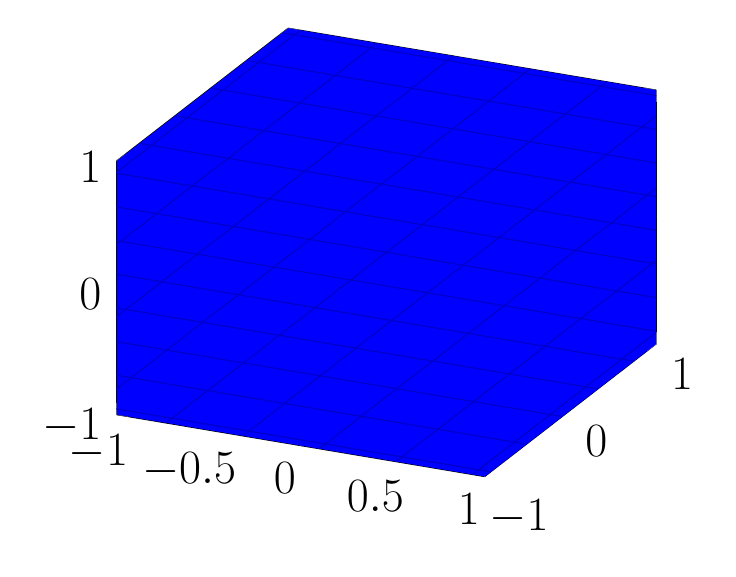
\begin{tikzpicture}
  \begin{axis}[xmin = -1, xmax = 1, ymin = -1, ymax = 1, zmin = -1, zmax = 1]
    \addplot3[variable = \z, surf] {x^2-y^2 == \z};
  \end{axis}
\end{tikzpicture}


\begin{tikzpicture}
 \begin{axis}[]
   \addplot[]{x^2};
   \addplot[only marks, point meta=explicit symbolic,] coordinates{(0, 10) [(1)]};
\end{axis}
\end{tikzpicture}

woo I can at least graph functions now


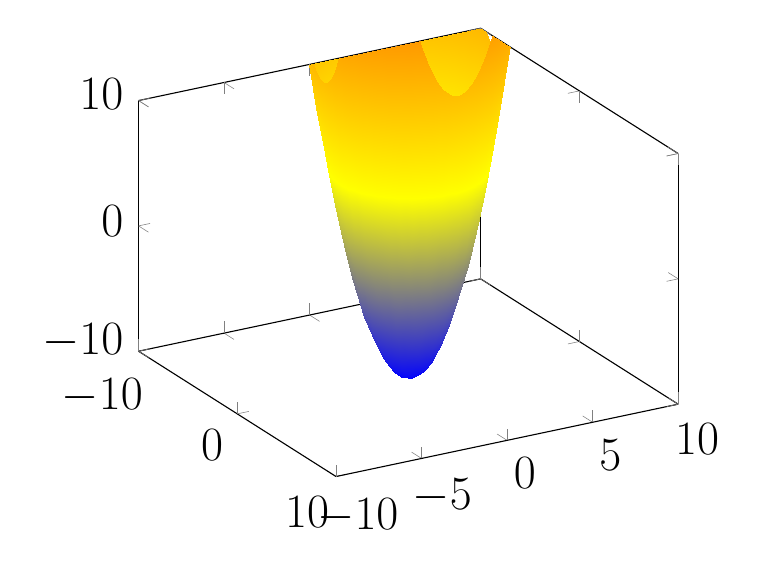
\begin{tikzpicture}
  \begin{axis}[xmin = -10, xmax = 10, ymin = -10, ymax = 10, zmin = -10, zmax = 10, view = {60}{30} ]
    \addplot3 [shader = interp, variable = z, surf, z buffer = sort]  {x^2+y^2-10};	
  \end{axis}
\end{tikzpicture}

This is a paraboloid this is $x^2 + y^2 -10 = z$
fucking shit this shits too complicated.



\end{document}